\documentclass{sosg-informe}

\graphicspath{{../../geodatos/estudios/la-cascada/figuras/}{figuras/}}

\title{La Cascada (Puerto Ayora):\\cuenca aportante, vaso cerrado\\y viabilidad del desvío de quebradas}
\titulocorto{La Cascada: cuenca, vaso y desvío}
\numero{2026-04}
\estado{Borrador para discusión}
\titulocita{La Cascada (Puerto Ayora): cuenca aportante, vaso cerrado y viabilidad del desvío de quebradas}
\relacionados{Issues \issue{2}, \issue{3}, \issue{16}, \issue{26} y \issue{65} · repositorio mayait/sosgalapagos-datos}
\date{4 de noviembre de 2026}

\begin{document}
\maketitle

\begin{abstract}
El 30 de octubre de 2026 una tormenta convectiva inundó el barrio La Cascada, en el norte de Puerto Ayora (Santa Cruz, Galápagos). Se pidió responder si es posible desviar las quebradas que bajan hacia el barrio. Con el modelo de superficie Copernicus GLO-30, la cartografía del IGM y OpenStreetMap se delimitó la cuenca aportante, se describió la depresión que ocupa el barrio y se buscaron corredores de desvío por gravedad. Los caudales se estimaron con el método SCS-CN y el hidrograma unitario SCS, con la tormenta tipo II y con la lluvia medida por la red IERSE-WSN aguas arriba. Al barrio drenan 42,3~km², casi toda la cuenca de Puerto Ayora, por dos quebradas que terminan en su borde norte. El barrio ocupa un \emph{vaso cerrado}: fondo a 10,5~m y rebose a 12,0--13,25~m según la definición (cota del DSM), con solo 42\,000--62\,000~m³ de almacenamiento y sin cauce de salida hacia el mar. Con la lluvia medida, la escorrentía del 30-oct fue de 46 a 92 veces ese volumen; el vaso se habría llenado horas antes del pico, y la altura del agua la controla la capacidad de salida, no el almacenamiento. Un interceptor a unos 40~m de cota hacia el este captaría el 99\,\% de la cuenca sin cruzar zonas pobladas, pero en sus primeros 2,5~km la pendiente es del orden del error del DSM, iría en terraplén o en corte profundo sobre el escarpe y quedaría entero en el Parque Nacional: el desvío \emph{no es descartable, pero no está demostrado}. Hacia el oeste no es viable. Todas las cifras son estimaciones de modelo sin calibrar con caudales ni con marcas de agua.
\palabrasclave{inundación pluvial; cuenca aportante; SCS-CN; hidrograma unitario; tiempo de concentración; depresión cerrada; desvío de cauces; Galápagos.}
\end{abstract}

\begin{aviso}
Este informe presenta \textbf{modelos propios, no datos oficiales}. No es un diseño de ingeniería, ni un mapa oficial de amenaza, ni un dictamen profesional. Las cotas son del DSM GLO-30, con un sesgo de $-2$ a $-3$~m frente al IGM, y no sirven como umbrales normativos; la cota real de rebose no está verificada (\issue{65}). El tránsito por el vaso (\enquote{bañera} más vertedero) no es un modelo hidráulico. El estudio lo preparó un comité de agentes de inteligencia artificial (asesor hidrológico, meteorología, gestión de riesgos y urbanismo) con un revisor independiente, sin visitas de campo ni revisión profesional externa; no expresa una posición institucional de la USFQ. Usa lluvia medida del IERSE (CC BY-NC-ND 4.0), lluvia de modelos meteorológicos, el DSM Copernicus GLO-30, cartografía del IGM, OpenStreetMap (ODbL) y capas del CGREG, la DPNG, el INEC y la SNGR; cada fuente conserva su licencia (\texttt{LICENCIA-DATOS.md}).
\end{aviso}

% =====================================================================
\section{Introducción}

Santa Cruz no tiene ríos permanentes. El agua de las lluvias fuertes baja desde la parte alta por quebradas secas y se concentra en pocos puntos de la costa. Uno de ellos es La Cascada, un barrio del norte de Puerto Ayora al pie del escarpe de una fosa tectónica. La tarde y la noche del 30 de octubre de 2026 el barrio se inundó; la SNGR registró daños en la UPC y en otros edificios públicos del sector, y el barrio ya figuraba en su registro de inundaciones de abril de 2023.

La coordinación de respuesta de USFQ Galápagos planteó una pregunta concreta: \emph{¿se pueden desviar las quebradas que bajan hacia La Cascada?} Responderla exige antes saber cuánta superficie drena al barrio, cuánta agua cabe en él, por dónde sale y en cuánto tiempo llega. Este informe documenta el análisis de gabinete hecho entre el 31 de octubre y el 2 de noviembre, y su recalibración posterior con la lluvia medida por la red IERSE-WSN. Es un reconocimiento: ordena las preguntas y las alternativas, pero no dimensiona obras.

El motor 2D que después se aplicó al mismo evento se documenta en el Informe técnico 2026-06 \citep{sosg202606}, y su uso para la alerta temprana, en el 2026-02 \citep{sosg202602}.

% =====================================================================
\section{Área de estudio y datos}

\subsection{El barrio}
El polígono del barrio, unión de las capas de OpenStreetMap y del CGREG, ocupa 6,1~ha. Su centroide está en $-90,3137$; $-0,7335$, a 0,94--1,25~km del mar. Las cotas del DSM van de 10,5 a 18,0~m, con una mediana de 13,1~m, frente a 22,7~m en un anillo de 300~m alrededor. Tiene 260 edificios (OSM y Google Open Buildings) y unas 1\,300 personas según las manzanas del INEC. Al norte se levanta un escarpe de 20--25~m, por encima del cual empieza el Parque Nacional Galápagos.

\subsection{Datos}
\begin{itemize}
  \item \textbf{Terreno:} DSM Copernicus GLO-30 \citep{esa2021}, reproyectado a UTM~15S en celdas de 30~m con interpolación bilineal. Incluye techos y copas de árboles. Frente a 468 puntos acotados del IGM 1:25\,000 situados a menos de 5~km del barrio, la diferencia media es de $-2,06$~m (RMSE 2,87~m); en zona poblada, $-3,38$~m (RMSE 3,81~m, $n = 53$).
  \item \textbf{Hidrografía y vías:} quebradas del IGM 1:25\,000 y de OSM; vías de OSM (31-oct-2026).
  \item \textbf{Exposición:} edificios de OSM y Google Open Buildings v3; población del INEC por manzana; viviendas de la SNGR.
  \item \textbf{Parque Nacional:} límite y zonificación de 2017 (DPNG y CGREG).
  \item \textbf{Lluvia medida [M]:} red IERSE-WSN de la Universidad del Azuay, pluviómetros de balancín de 0,2~mm con registros cada ${\sim}5$~min en hora de Galápagos. Dos estaciones útiles el 30-oct, ambas fuera de la cuenca (tabla~\ref{tab:lluvia}). \textbf{No hubo lluvia medida dentro de Puerto Ayora incorporada al estudio}: la estación INAMHI M0191, a 1,4~km del barrio, registró el evento, pero su serie aún no se ha integrado (\issue{3}).
  \item \textbf{Lluvia de modelos [E]:} ECMWF IFS (9~km y 0,25°), GFS, ICON, UKMO, Météo-France, JMA y ERA5, obtenidos el 2-nov.
  \item \textbf{Climatología [M]:} lluvia diaria de la Fundación Charles Darwin en Puerto Ayora y Bellavista.
\end{itemize}

\begin{table}[ht]
  \centering\small
  \caption{Lluvia medida el 30 de octubre de 2026 por la red IERSE-WSN (hora UTC$-6$). Los totales son mínimos: las dos estaciones útiles dejaron de transmitir cuando todavía llovía.}
  \label{tab:lluvia}
  \begin{tabularx}{\linewidth}{>{\raggedright\arraybackslash}Xccccc}
    \toprule
    Estación & Cota & Total 30-oct & Máx. en 1~h & Último registro & Uso \\
    \midrule
    Los Guayabillos (parte media, a 370~m de la cuenca) & 178~m & 178,8~mm & 61,0~mm & 21:25 & central \\
    Santa Rosa (oeste, fuera de la cuenca) & 416~m & 237,6~mm & 66,4~mm & 21:22 & gradiente \\
    Cerro Crocker (cumbre) & 861~m & 5,0~mm & 0,8~mm & 23:57 & descartada \\
    Militar (Baltra) & 14~m & 2,0~mm & 0,8~mm & 23:57 & --- \\
    \bottomrule
  \end{tabularx}
  \par\vspace{3pt}\raggedright\footnotesize Cerro Crocker casi seguro falla desde agosto: midió 9 y 18~mm en septiembre y octubre frente a 140 y 340~mm en Los Guayabillos. Los Guayabillos marca 0~mm del 31-oct al 2-nov mientras Santa Rosa mide 13--43~mm al día; su registro del 30-oct es coherente con el de Santa Rosa y se mantiene.
\end{table}

% =====================================================================
\section{Métodos}

\subsection{Cuenca aportante}
La dirección de flujo se calculó con el método D8 \citep{ocallaghan1984}, con \texttt{pysheds} \citep{bartos2020}, sobre el DSM con las quebradas del IGM \enquote{quemadas}, tras rellenar depresiones y resolver zonas planas. Cada celda se asignó a la entrada por la que su flujo alcanza primero el barrio, lo que separa dos ramas y la escorrentía local. Como control, la cuenca se recalculó sin quemar las quebradas.

\subsection{Tiempo de concentración}
Se usaron dos fórmulas empíricas sobre el cauce principal, de longitud $L$ y pendiente media $S$ (m/m). La de Kirpich \citep{kirpich1940}, con $L$ en metros, y la de Témez \citep{temez1978}, con $L$ en kilómetros:
\begin{equation}
  t_{c,\mathrm{K}}\,[\mathrm{min}] = 0,0195\, L^{0,77}\, S^{-0,385},
  \qquad
  t_{c,\mathrm{T}}\,[\mathrm{h}] = 0,3 \left(\frac{L}{S^{1/4}}\right)^{0,76}.
  \label{eq:tc}
\end{equation}
Como contraste se calcularon el retardo SCS en función del CN, la suma de velocidades de flujo superficial de TR-55 \citep{usda1986} y la velocidad de Manning en el cauce. La fórmula de California Culverts Practice es algebraicamente la de Kirpich y no se cuenta como método independiente.

\subsection{Lluvia efectiva e hidrograma}
La escorrentía acumulada $Q$ (mm) se obtiene de la lluvia acumulada $P$ con el número de curva \citep{usda1986}:
\begin{equation}
  S = \frac{25\,400}{\mathrm{CN}} - 254, \qquad I_a = 0,2\,S, \qquad
  Q = \begin{cases} \dfrac{(P - I_a)^2}{P - I_a + S} & P > I_a \\[4pt] 0 & P \leq I_a \end{cases}
  \label{eq:scs}
\end{equation}
El CN compuesto pondera tres coberturas con valores supuestos: Parque (lava con suelo somero), 55; zona agrícola, 76; zona poblada, 90. Las condiciones seca y húmeda se obtienen con las relaciones habituales \citep{chow1988}:
\begin{equation}
  \mathrm{CN}_{\mathrm{I}} = \frac{4,2\,\mathrm{CN}_{\mathrm{II}}}{10 - 0,058\,\mathrm{CN}_{\mathrm{II}}}, \qquad
  \mathrm{CN}_{\mathrm{III}} = \frac{23\,\mathrm{CN}_{\mathrm{II}}}{10 + 0,13\,\mathrm{CN}_{\mathrm{II}}}.
\end{equation}
El exceso de cada paso de $\Delta t = 10$~min se convoluciona con el hidrograma unitario adimensional del SCS, con tiempo al pico
\begin{equation}
  t_p = \frac{\Delta t}{2} + 0,6\, t_c ,
\end{equation}
escalado para que el volumen sea exacto. La cuenca es agregada, con lluvia uniforme, sin flujo base ni tránsito por cauces. Se usaron tres entradas de lluvia:
\begin{itemize}
  \item \textbf{Diseño:} tormenta SCS tipo II de 24~h \citep{usda1986}, con 50, 100, 150 y 200~mm y CN de 60, 70 y 80.
  \item \textbf{Evento modelado [E] (versión del 2-nov):} hietograma horario de ECMWF IFS 9~km en una celda costera y otra alta, ponderadas por la fracción de la cuenca sobre 200~m (0,55). Las etiquetas venían en hora continental (UTC$-5$) y se pasaron a UTC$-6$.
  \item \textbf{Evento medido [M] (recalibración):} hietograma de 10~min de la red IERSE-WSN, con tres variantes de lluvia areal: Los Guayabillos uniforme (central); la misma serie por un factor de reducción areal de 0,85, tomado de las curvas TP-29 para 1--3~h y unos 40~km² \citep{tp29} (cota inferior); e interpolación lineal con la cota entre Los Guayabillos (178~m) y Santa Rosa (416~m), constante fuera de ese intervalo (cota superior).
\end{itemize}

\subsection{Vaso y curva cota--volumen (\enquote{bañera})}
Sobre el DSM sin quemar se hizo un llenado estático: para cada cota $h$ se toman las celdas con cota $\leq h$ conectadas en 8 vecinos con el punto más bajo del barrio, dentro de un radio de 600~m. El volumen es
\begin{equation}
  V(h) = \sum_{i \in \Omega(h)} (h - z_i)\, A_c, \qquad A_c = 900~\mathrm{m}^2 .
\end{equation}
El llenado no tiene caudal, tiempo ni pérdidas: \textbf{no es un modelo hidráulico}. La exposición se cuenta con los edificios que tocan la mancha o que tienen su centroide dentro, y con la población del INEC ponderada por área.

\subsection{Rebose: camino de mínimo umbral}
La cota de rebose es la mínima cota de lámina a la que el agua conectada al punto bajo alcanza el mar. Se calcula con una búsqueda de tipo Dijkstra \citep{dijkstra1959} que, en lugar de la distancia, minimiza la cota máxima encontrada a lo largo del camino (\emph{minimax}), con desempate por longitud:
\begin{equation}
  h_{\mathrm{reb}} = \min_{\gamma:\ p_0 \to \text{mar}}\ \max_{i \in \gamma} z_i .
\end{equation}
Se probaron cuatro variantes: DSM o \enquote{proxy de suelo} (mínimo del DSM en una ventana de $3 \times 3$ celdas, que atenúa los techos), con 4 u 8 vecinos. La de referencia es el DSM con 8 vecinos; las demás acotan la incertidumbre.

\subsection{Tránsito por el vaso}
Para el evento medido, el hidrograma de entrada se transitó por el vaso con la curva cota--volumen y una salida en vertedero de cresta ancha sobre el umbral de rebose \citep{chow1959}:
\begin{equation}
  \frac{\mathrm{d}V}{\mathrm{d}t} = Q_{\mathrm{in}}(t) - C\, L_w \,\bigl[\max(0,\ h - h_{\mathrm{reb}})\bigr]^{3/2}, \qquad C = 1,7~\mathrm{m^{1/2}/s},
  \label{eq:vertedero}
\end{equation}
con paso de 1~min. La longitud efectiva del frente de desborde $L_w$ se desconoce y se toma como 100, 300 y 1\,000~m. El vertedero libre ignora el remanso aguas abajo.

\subsection{Corredores de desvío}
Los corredores se buscaron con una variante de Dijkstra que maximiza la cota de la rasante del canal. Desde la toma, la rasante debe bajar al menos 0,5\,\% por metro; puede ir hasta 1~m sobre el terreno (terraplén) o hasta 3~m bajo él (6~m como sensibilidad), y no puede pasar por zonas pobladas, manzanas ni barrios, con un margen de 30~m. Se probaron tomas a 20, 30, 40, 60, 80 y 120~m en las dos ramas, con salida al oeste, al frente urbano o al este: 24 combinaciones. El área captada es la de las celdas de la cuenca cuyo flujo D8 cruza la traza antes de llegar al barrio. El ancho de base de un canal trapecial (talud 1:1, calado 2,5~m, $n = 0,035$) se obtuvo con Manning.

% =====================================================================
\section{Resultados}

\subsection{Cuenca aportante y tiempos}
Al barrio drenan \textbf{42,3~km²}, casi toda la cuenca de Puerto Ayora (tabla~\ref{tab:cuenca}, figura~\ref{fig:cuenca}). El resultado es idéntico sin quemar las quebradas, y solo el 0,7\,\% del área depende de depresiones rellenadas de más de 1~m: la conexión no es un artefacto del relleno. Las quebradas del IGM terminan en el borde norte del barrio. Las dos ramas miden unos 13,0~km por coincidencia geométrica: nacen en cabeceras distintas de la divisoria (773 y 806~m).

\begin{table}[ht]
  \centering\small
  \caption{Subcuencas que drenan a La Cascada y tiempo de concentración del cauce principal (ecuación~\ref{eq:tc}).}
  \label{tab:cuenca}
  \begin{tabular}{lcccccc}
    \toprule
    Subcuenca & Área & Cota máx. & \makecell{Pendiente\\media} & \makecell{Cauce\\(longitud, pendiente)} & \makecell{$t_c$\\Kirpich} & \makecell{$t_c$\\Témez} \\
    \midrule
    Rama 1 (norte) & 29,5~km² & 856~m & 10,1\,\% & 13,0~km; 5,8\,\% & 1,43~h & 3,61~h \\
    Rama 2 (noroeste) & 12,2~km² & 826~m & 9,2\,\% & 13,0~km; 6,1\,\% & 1,40~h & 3,58~h \\
    Escorrentía local & 0,6~km² & 65~m & 5,9\,\% & --- & --- & --- \\
    \midrule
    Total & 42,3~km² & & 9,7\,\% & & & \\
    \bottomrule
  \end{tabular}
\end{table}

\begin{figure}[tp]
  \centering
  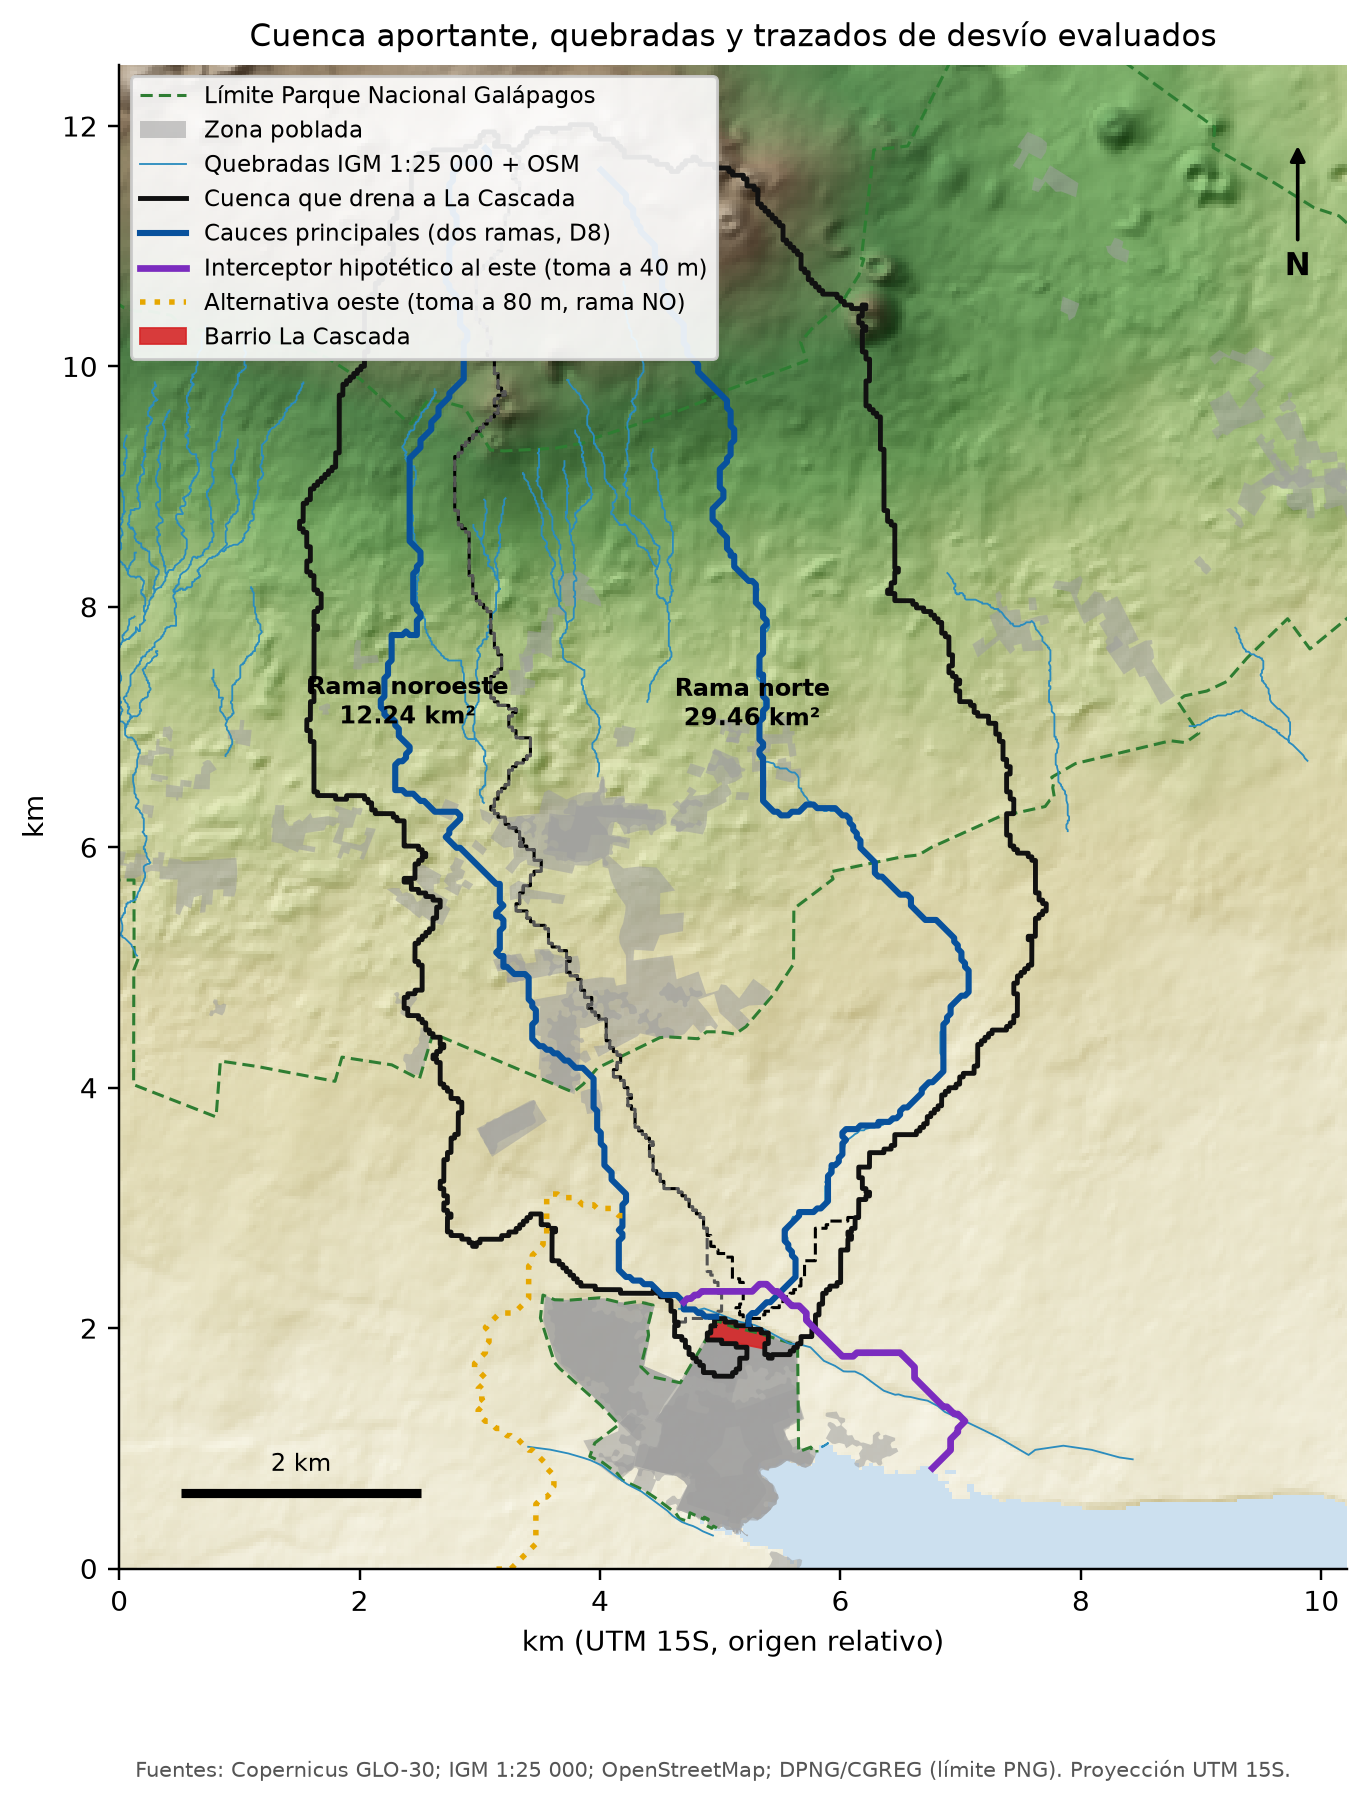
\includegraphics[height=0.62\textheight]{f_mapa_cuenca.png}
  \caption{Cuenca que drena a La Cascada (42,3~km²), con sus dos ramas (cauces D8), las quebradas del IGM y de OSM, el límite del Parque Nacional y los trazados de desvío evaluados: interceptor hipotético al este (toma a 40~m, morado) y alternativa oeste (toma a 80~m, naranja). Fuentes: Copernicus GLO-30, IGM 1:25\,000, OSM, DPNG/CGREG.}
  \label{fig:cuenca}
\end{figure}

Para toda la cuenca, Kirpich da 1,4~h, la velocidad de Manning en el cauce 1,5~h, Témez 3,6~h, TR-55 4,2~h y el retardo SCS 3,4--5,9~h (CN 80 a 60). Kirpich se calibró en cuencas agrícolas de menos de 0,5~km², y el retardo SCS en cuencas de menos de unos 8~km²; ambos quedan fuera de rango. Se adopta \textbf{Témez (3,6~h) como valor central} y Kirpich como cota superior del caudal pico; el intervalo defendible es de 1,4 a 5,9~h. En términos operativos, una crecida que pasa por el cauce de Bellavista (cota 170~m, 8,1~km² drenados) tardaría de 65 (Kirpich) a 142~min (Témez) en llegar al barrio, y desde el borde del escarpe (cota 40~m) de 5 a 18~min. Son tiempos de concentración, no tiempos de viaje medidos.

\subsection{Un vaso cerrado al pie de escarpes}
Las secciones transversales muestran un fondo cerrado por tres lados (figura~\ref{fig:secciones}): al norte el terreno cae de unos 36 a 13~m en 240~m; al este hay un escalón de 29 a 12,5~m en 120~m; al oeste sube a 26--28~m. El punto más bajo está a 10,53~m ($-90,31452$; $-0,73401$).

\begin{figure}[tp]
  \centering
  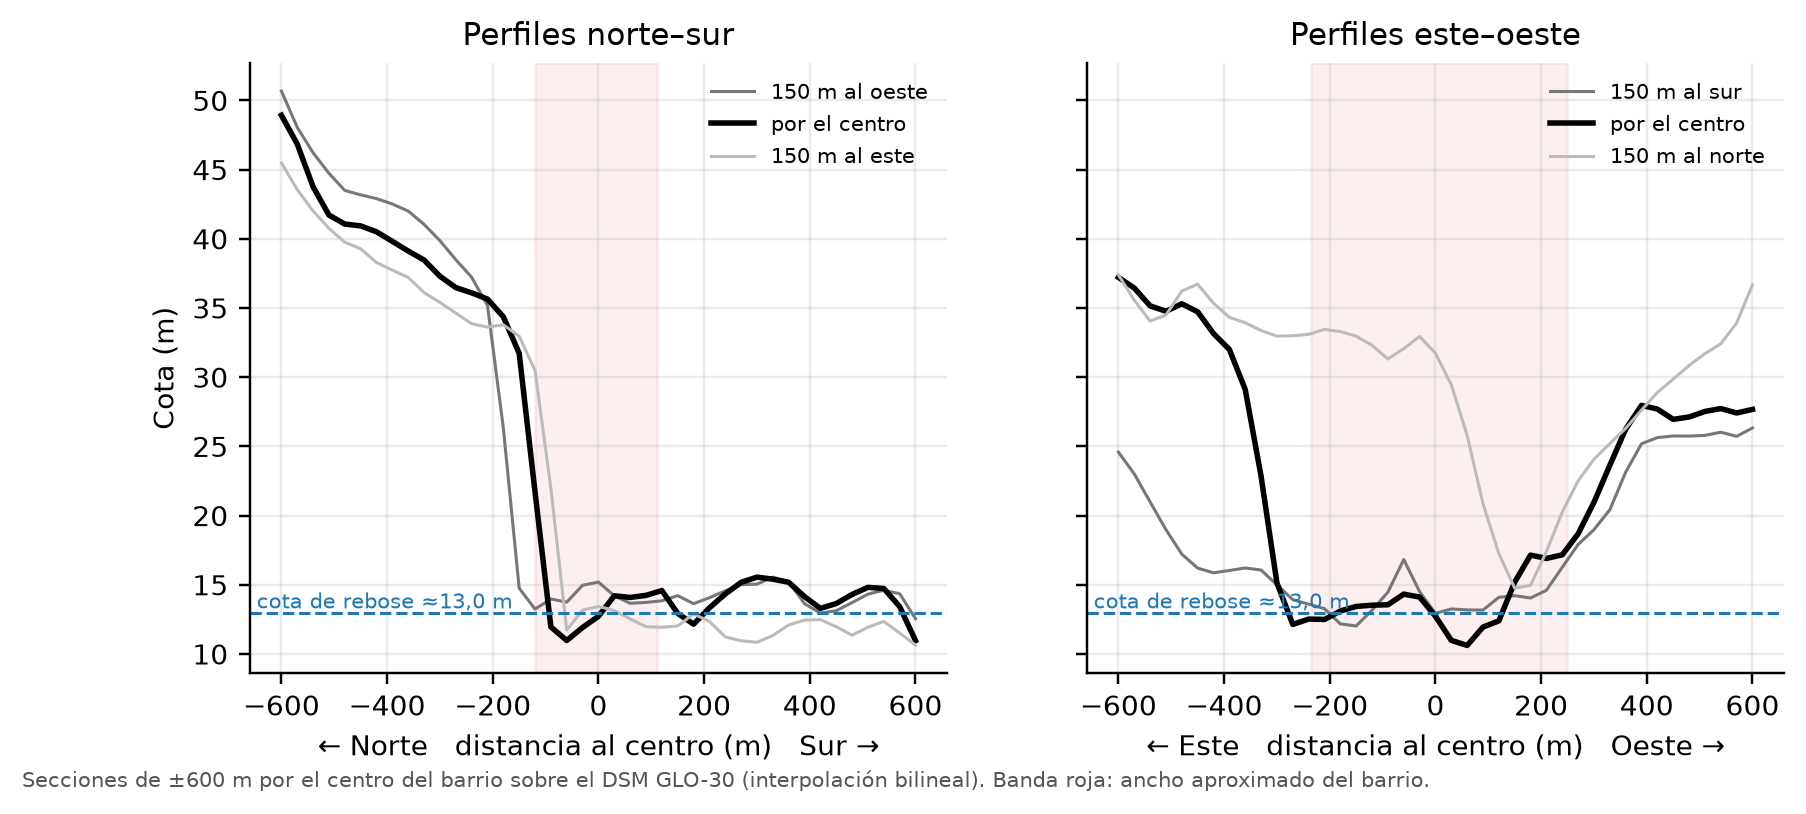
\includegraphics[width=\linewidth]{f_secciones.png}
  \caption{Perfiles norte--sur y este--oeste de $\pm 600$~m por el barrio (DSM, interpolación bilineal). La línea discontinua marca la cota de rebose del vaso.}
  \label{fig:secciones}
\end{figure}

La cota de rebose de referencia es \textbf{12,95~m} (DSM, 8 vecinos), con el punto de control unos 270~m al ESE del punto bajo ($-90,31237$; $-0,73509$). Con 4 vecinos sube a 13,25~m, y con el proxy de suelo baja a 12,0~m. El umbral del proxy de suelo coincide con un lomo de unos 1,3--1,4~m sobre la línea de flujo urbana, en las calles Isla Santiago y Karl Angermeyer, cuyo origen (lava o relleno) no se distingue a 30~m. \textbf{La cota real del rebose está entre unos 12,0 y 13,25~m y solo puede fijarse con GNSS} (\issue{65}).

Hasta el rebose, el vaso almacena \textbf{42\,000--62\,000~m³ en 3,7--6,2~ha}, con 2,4~m de profundidad máxima. El rango depende de si un paso diagonal a ${\approx}\,12,85$~m une una segunda poza (8 frente a 4 vecinos). Otro criterio, que sumaba todas las depresiones de más de 0,2~m a menos de 400~m, daba 14~ha y 125\,000~m³; el cálculo se reprodujo, pero agrupa 19 vasos independientes con cotas de rebose de 11,4 a 34,9~m, así que no representa el almacenamiento del barrio.

\begin{table}[ht]
  \centering\small
  \caption{Curva cota--volumen--exposición del llenado estático (\enquote{bañera}) conectado al punto bajo, dentro de un radio de 600~m. Edificios de OSM y Open Buildings que tocan la mancha; población del INEC ponderada por área.}
  \label{tab:curva}
  \begin{tabular}{cccccc}
    \toprule
    Cota (m, DSM) & Área & Volumen & Edificios & Población estimada & ¿Sobre el rebose? \\
    \midrule
    12,0 & 1,7~ha & 11\,700~m³ & 66 & 283 & no \\
    12,5 & 2,3~ha & 21\,700~m³ & 86 & 400 & no \\
    13,0 & 13,2~ha & 138\,800~m³ & 406 & 1\,458 & sí \\
    13,5 & 21,2~ha & 261\,600~m³ & 630 & 2\,149 & sí \\
    14,0 & 25,7~ha & 379\,900~m³ & 782 & 2\,759 & sí \\
    15,0 & 39,9~ha & 733\,900~m³ & 1\,162 & 4\,251 & sí \\
    16,0 & 46,4~ha & 1\,168\,400~m³ & 1\,317 & 4\,965 & sí \\
    \bottomrule
  \end{tabular}
  \par\vspace{3pt}\raggedright\footnotesize Por encima de 12,95~m la mancha ya no es agua almacenada: describe el camino del desborde hasta el borde de la ventana de cálculo, y solo se sostendría con la salida en remanso u obstruida. Esas filas no deben citarse como exposición.
\end{table}

Dentro del vaso, entre 12,5~m y el rebose, quedan \textbf{68--204 edificios, unas 400--910 personas y 74--182 viviendas} (tabla~\ref{tab:curva}, figura~\ref{fig:curva}). El mínimo cuenta los edificios por su centroide a 12,5~m; el máximo, los que tocan la mancha justo bajo el rebose con 8 vecinos.

\begin{figure}[tp]
  \centering
  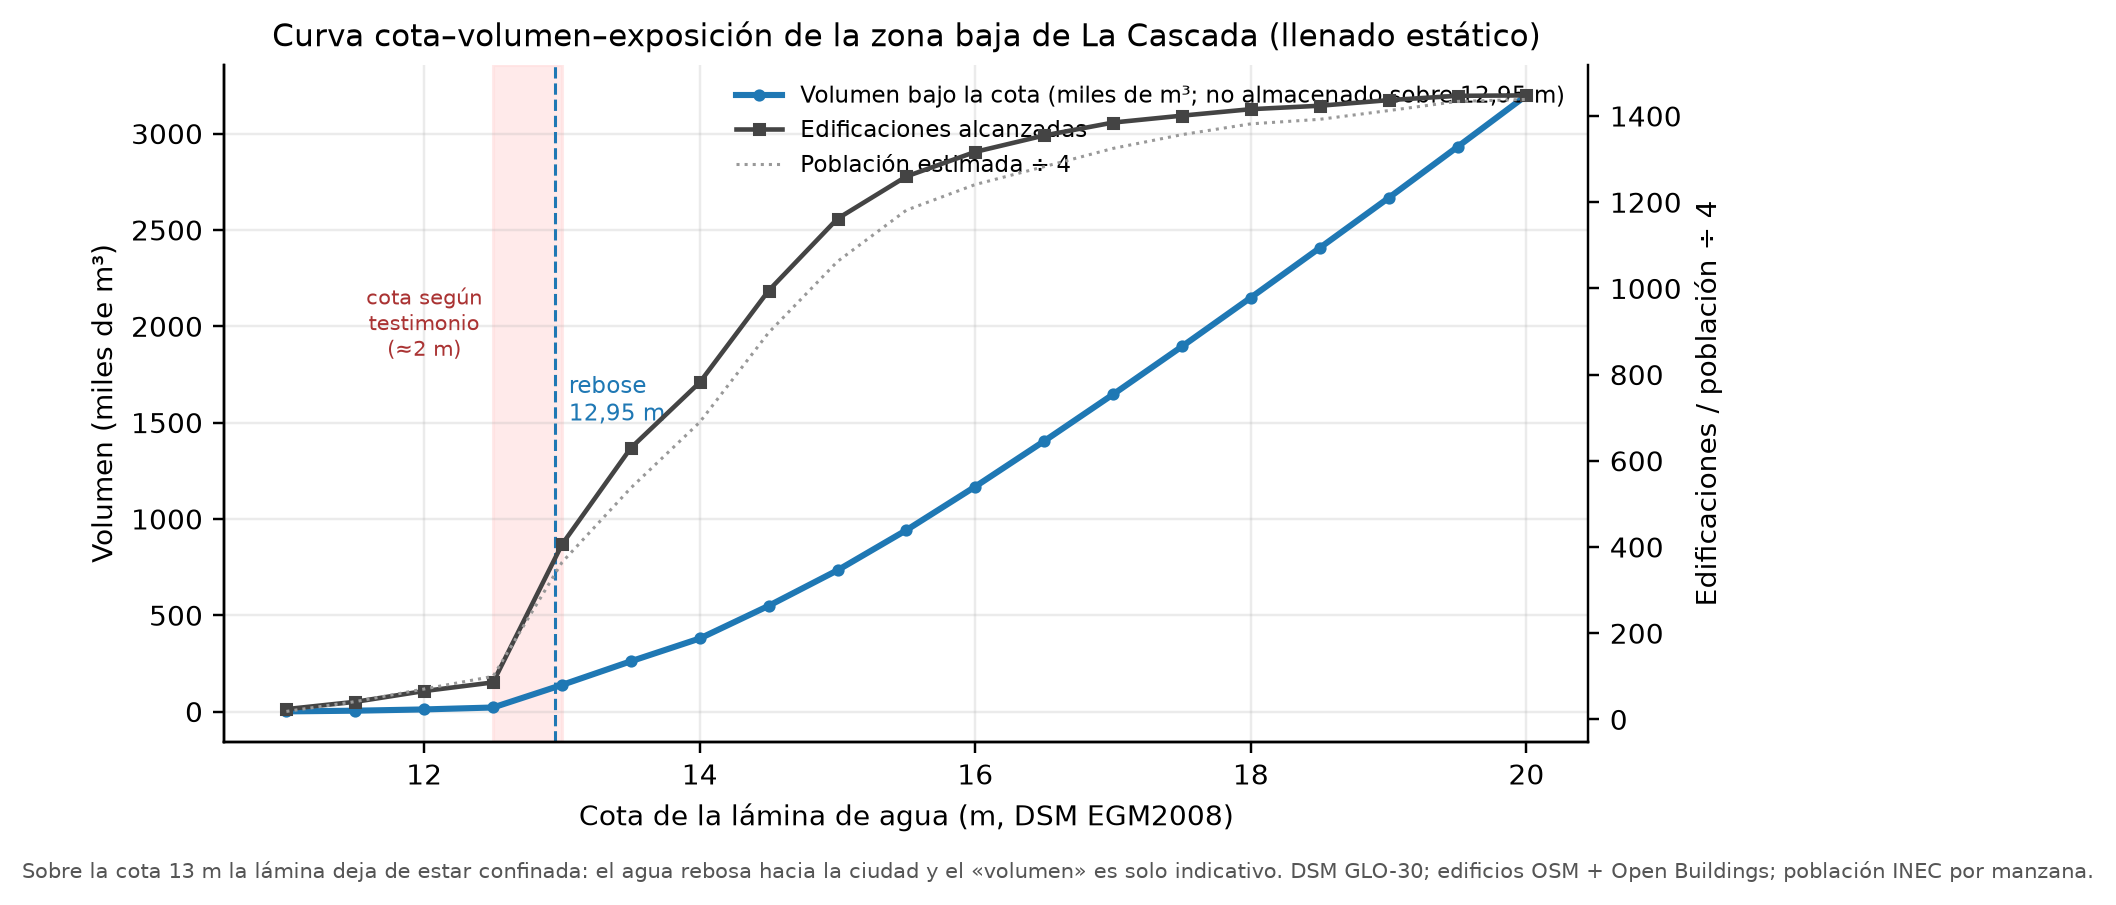
\includegraphics[width=\linewidth]{f_cota_volumen.png}
  \caption{Curva cota--volumen--exposición de la zona baja (llenado estático conectado). La banda marca el intervalo de cota compatible con el único testimonio con fuente (agua \enquote{hasta dos metros}, prensa, por validar).}
  \label{fig:curva}
\end{figure}

\subsection{El agua no tiene cauce de salida}
El camino de mínimo umbral cruza los 12,95~m y se divide en dos ramas: al \textbf{sur}, 1,5~km hasta la bahía, con el 94\,\% del recorrido en zona poblada y 208 edificios a menos de 20~m; al \textbf{este}, por el fondo de la fosa, 2,2~km, con el 76\,\% en zona poblada y 185 edificios. Entre el barrio y el mar no hay ningún cauce cartografiado. La línea de flujo D8 recorre 1\,194~m hacia el SSE, de 12,0 a 1,3~m (0,9\,\% de pendiente media): los primeros 400~m son casi planos, pasa sobre 28 edificaciones y cruza 16 veces una vía. Según la prensa (2023, sin fuente oficial), Santa Cruz no tiene alcantarillado pluvial.

OSM dibuja un cauce intermitente de 4,1~km al pie del escarpe hacia el ESE, sin nombre ni fuente; el IGM no cartografía nada allí. Su perfil es coherente en los primeros 480~m, pero después el mínimo de una franja de $\pm 90$~m sube en cuatro umbrales (18,8; 17,8; 21,2 y 33,0~m), y su extremo oriental queda a 42~m de cota y a 370~m de la costa. Para recorrerlo entero el agua tendría que subir a 36,9~m, frente a los 12,95~m del rebose: \textbf{tal como está dibujado, no es un cauce hidráulicamente coherente}.

\subsection{Hidrogramas de diseño}
La cuenca se reparte en un 42\,\% de Parque, un 50\,\% de zona agrícola y un 8\,\% de zona poblada. El CN compuesto es 68,3 en condición normal, 47,4 en seca y 83,2 en húmeda. La tabla~\ref{tab:diseno} resume los escenarios de diseño.

\begin{table}[ht]
  \centering\small
  \caption{Escenarios de diseño: tormenta SCS tipo II de 24~h sobre 42,4~km² (cuenca más barrio). La última columna divide el volumen por el vaso máximo de 62\,000~m³.}
  \label{tab:diseno}
  \begin{tabular}{cccccc}
    \toprule
    \makecell{Lluvia\\24~h} & CN & \makecell{Escorrentía\\(mm)} & \makecell{$Q_p$ Témez\\(m³/s)} & \makecell{$Q_p$ Kirpich\\(m³/s)} & \makecell{Volumen /\\vaso} \\
    \midrule
    50~mm & 60 / 70 / 80 & 1,4 / 5,8 / 13,8 & 1,5 / 10 / 30 & 1,7 / 17 / 58 & 1 / 4 / 9 \\
    100~mm & 60 / 70 / 80 & 18,6 / 32,7 / 50,5 & 36 / 74 / 123 & 67 / 143 / 239 & 13 / 22 / 35 \\
    150~mm & 60 / 70 / 80 & 47 / 69 / 94 & 106 / 167 / 232 & 205 / 324 / 448 & 32 / 47 / 64 \\
    200~mm & 60 / 70 / 80 & 82 / 111 / 140 & 195 / 272 / 347 & 378 / 526 / 664 & 56 / 76 / 96 \\
    \bottomrule
  \end{tabular}
\end{table}

Según el SCS-CN agregado, y suponiendo que toda la escorrentía llega al barrio sin pérdidas en los cauces efímeros, el vaso se llenaría con unos 25--50~mm. \textbf{La lluvia medida en octubre no respalda ese resultado}: el 3-oct cayeron 68,2~mm en Los Guayabillos (112~mm entre el 3 y el 4) con un máximo horario de 12,6~mm/h, sin inundación reportada en el barrio (por confirmar, \issue{52}). El 30-oct hubo unas tres horas seguidas a 21--61~mm/h. La diferencia está en la \emph{intensidad}: el umbral empírico estaría del orden de 20--25~mm/h sostenidos más de una hora sobre la parte media de la cuenca. El SCS-CN reparte las pérdidas según el volumen acumulado, no según la intensidad, y sobrestima la frecuencia de llenado; el modelo 2D con pérdida constante sí separa los dos días \citep{sosg202606}.

\subsection{El evento del 30 de octubre}
\textbf{Versión con lluvia de modelo (2-nov).} Antes de disponer de la serie IERSE, el evento se representó con ECMWF IFS 9~km: 110~mm ponderados (82~mm en la celda costera, 133~mm en la alta), con el máximo hacia las 05:00--06:00 del 31-oct. Con CN 76 daba 119--186~m³/s (Témez--Kirpich) a las 06:30--07:30 del 31-oct, y 87--245~m³/s en el rango de CN 68--83. Los demás modelos daban entre 0,2 y 26~mm ese día; ECMWF de 0,25° (26~mm ponderados) produce unos 1~m³/s. Ningún modelo está validado en la isla.

\textbf{Recalibración con lluvia medida.} La lluvia medida sitúa el núcleo del evento entre las 18:00 y las 21:30 del 30-oct, ocho a nueve horas antes que ECMWF, y coincide con la \enquote{tarde y noche del 30} que reporta la SNGR. ECMWF queda descartado como representación del evento. La tabla~\ref{tab:evento} y la figura~\ref{fig:hidrogramas} resumen los hidrogramas con CN 76, el valor central: los 5 días previos sumaron solo 10--12~mm (AMC I--II), pero octubre fue húmedo y el mismo día ya habían caído unos 25~mm antes del pulso principal. CN 68 es igual de defendible; CN 83 queda sin respaldo.

\begin{table}[ht]
  \centering\small
  \caption{Hidrogramas del evento medido del 30-oct en la entrada al barrio (CN 76; intervalos Témez--Kirpich; hora UTC$-6$). Modelo agregado sin calibrar con caudales.}
  \label{tab:evento}
  \setlength{\tabcolsep}{4pt}\footnotesize
  \begin{tabular}{lcccccc}
    \toprule
    Lluvia areal & \makecell{Escorrentía\\(C)} & Volumen & \makecell{Veces\\el vaso} & \makecell{$Q_p$\\(m³/s)} & \makecell{Hora\\del pico} & \makecell{Vaso lleno\\a las} \\
    \midrule
    Reducción areal, 152~mm & 85~mm (0,56) & 3,59~hm³ & 58 & 260--401 & 21:40--22:50 & 17:45--19:10 \\
    \textbf{Los Guayabillos, 179~mm} & \textbf{108~mm (0,61)} & \textbf{4,59~hm³} & \textbf{74} & \textbf{325--497} & \textbf{21:40--22:50} & \textbf{16:50--18:10} \\
    Gradiente con la cota, 208~mm & 134~mm (0,65) & 5,69~hm³ & 92 & 362--549 & 21:30--22:40 & 15:40--16:30 \\
    \bottomrule
  \end{tabular}
  \par\vspace{3pt}\raggedright\footnotesize Con CN 76 el caudal supera 1~m³/s desde las 10:30--16:20, según el escenario. Con CN 68 el pico central queda en 277--434~m³/s, y el volumen en 46 veces el vaso con reducción areal. El conjunto de escenarios (152--208~mm, CN 68--76) da 215--549~m³/s, o 5--13~m³/s por km².
\end{table}

\begin{figure}[t]
  \centering
  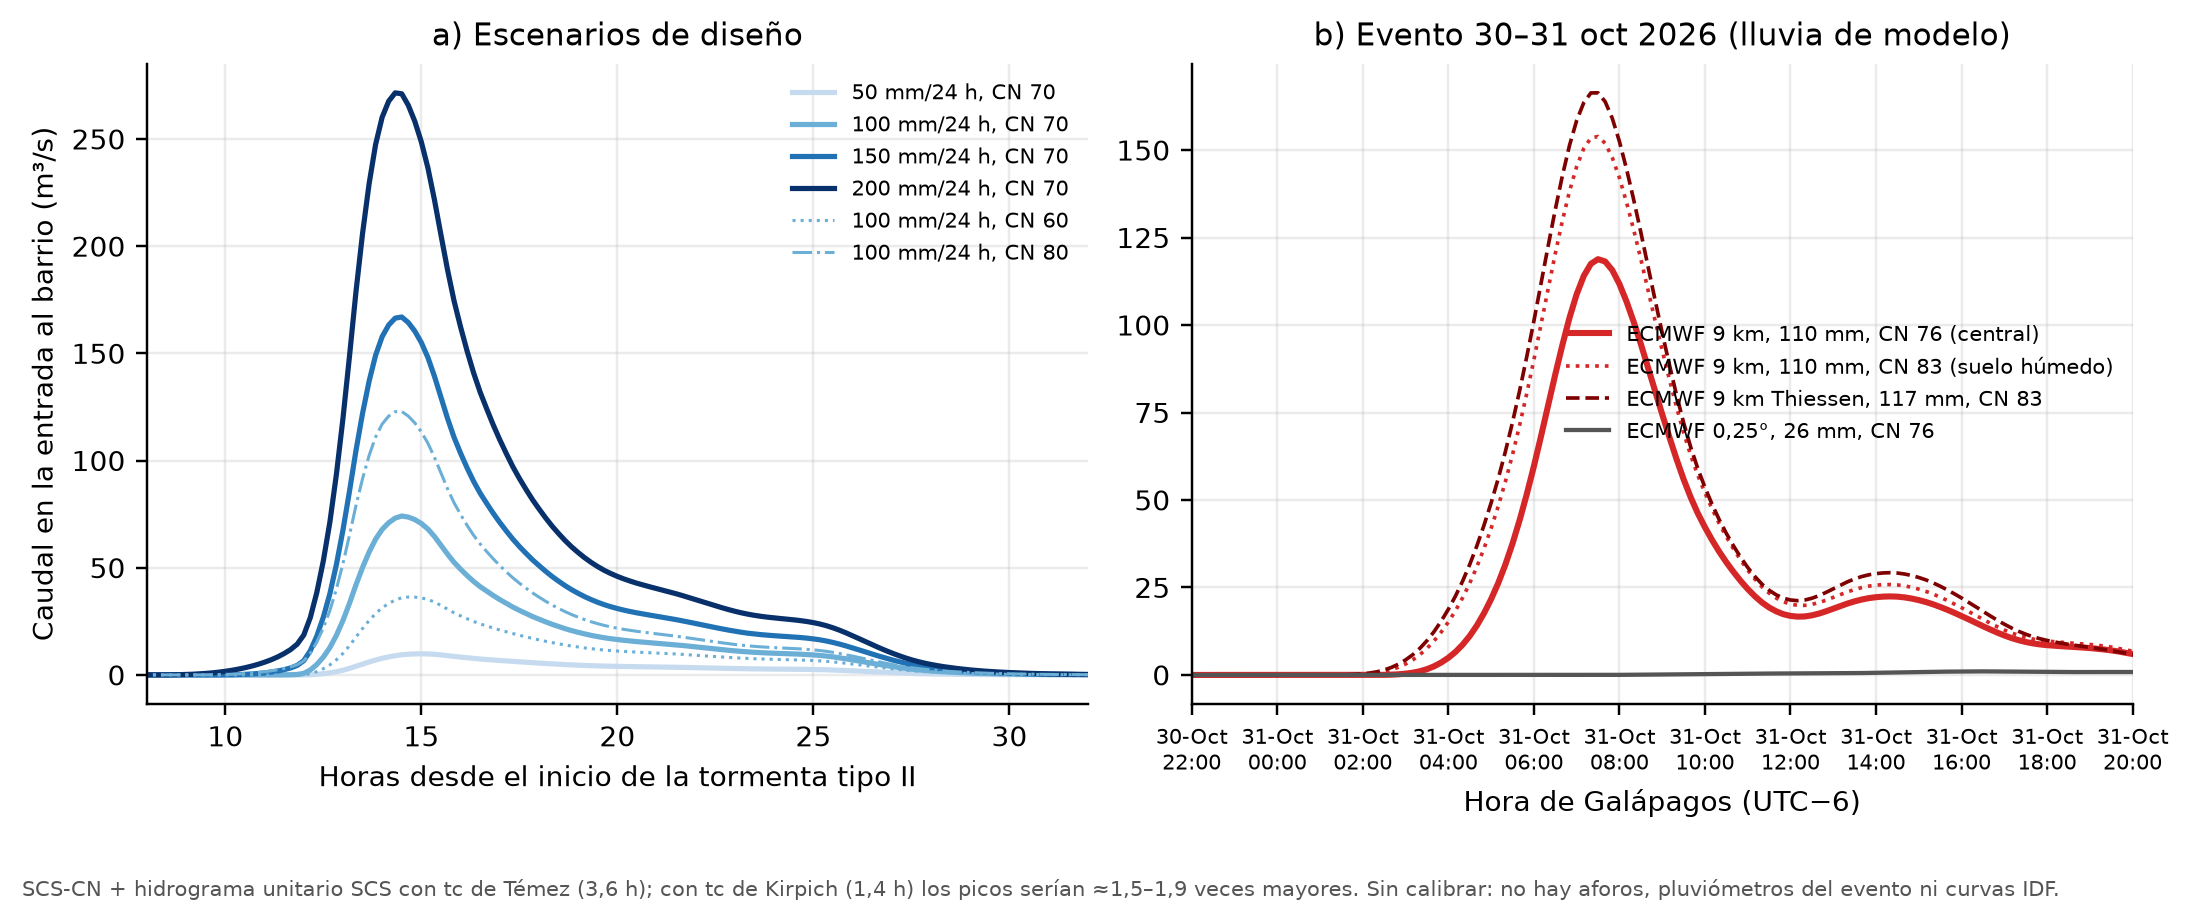
\includegraphics[width=\linewidth]{f_hidrogramas.png}
  \caption{Hidrogramas sintéticos SCS-CN en la entrada al barrio. (a) Escenarios de diseño con tormenta tipo II de 24~h. (b) Evento del 30-oct con la lluvia medida por la red IERSE-WSN: tres variantes de lluvia areal con CN 76, y la lluvia horaria de Los Guayabillos (eje derecho). La línea punteada vertical marca el fin del registro (21:25).}
  \label{fig:hidrogramas}
\end{figure}

\textbf{Tránsito por el vaso.} Con la ecuación~\ref{eq:vertedero}, la cota máxima del agua va de 13,2 a 15,1~m según la longitud del frente de desborde (tabla~\ref{tab:transito}, figura~\ref{fig:transito}). Lo que más la cambia es $L_w$, no la lluvia ni el CN: con un frente de 300~m todos los escenarios con CN 68--76 caen entre 13,5 y 14,0~m, porque la lámina la fija la cota del umbral más una carga que crece con $Q^{2/3}$. El vaso vuelve a la cota de rebose entre las 00:00 y las 08:00 del 31-oct; por debajo quedan retenidos 42\,000--62\,000~m³ sin salida por gravedad.

\begin{table}[ht]
  \centering\small
  \caption{Lámina máxima simulada sobre el punto más bajo del DSM (10,53~m) con el tránsito por el vaso: lluvia areal de 152--208~mm, CN 68--76 y $t_c$ de Témez a Kirpich.}
  \label{tab:transito}
  \begin{tabular}{cccc}
    \toprule
    Frente de desborde $L_w$ & Cota máxima del agua & Lámina sobre el fondo & Hora de la lámina máxima \\
    \midrule
    100~m & 14,1--15,1~m & 3,6--4,5~m & 21:50--23:10 \\
    300~m & 13,5--14,0~m & 3,0--3,5~m & 21:40--23:00 \\
    1\,000~m & 13,2--13,4~m & 2,7--2,9~m & 21:40--22:55 \\
    \bottomrule
  \end{tabular}
\end{table}

\begin{figure}[t]
  \centering
  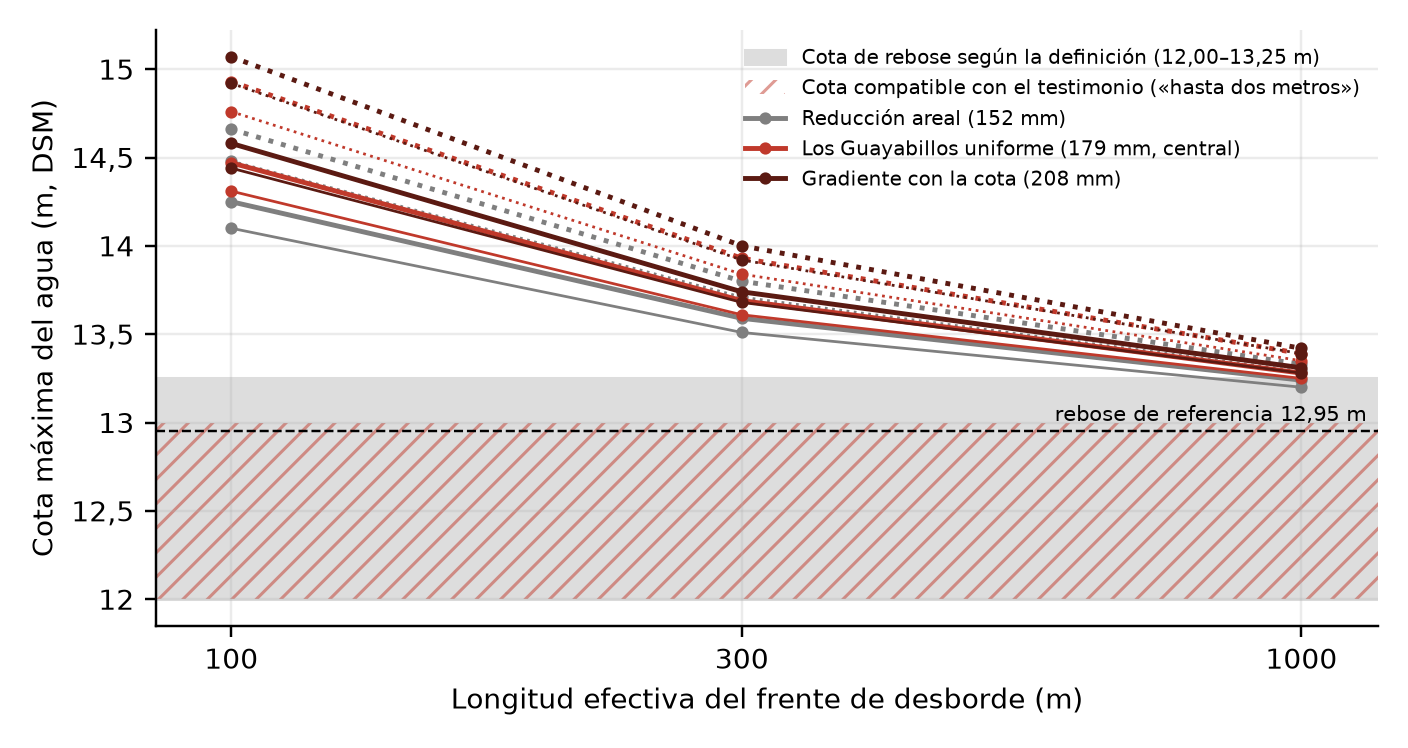
\includegraphics[width=0.86\linewidth]{transito_vaso.png}
  \caption{Cota máxima del agua en el vaso según la longitud efectiva del frente de desborde, para las tres lluvias areales del 30-oct. Línea gruesa: CN 76; fina: CN 68. Continua: $t_c$ de Témez; punteada: Kirpich. Banda gris: cota de rebose según la definición; rayado: cota compatible con el testimonio. Figura nueva, generada con \texttt{figuras.py} a partir de \texttt{resumen.json}.}
  \label{fig:transito}
\end{figure}

\textbf{Comparación con lo observado.} El único dato con fuente es el testimonio de agua \enquote{hasta dos metros} (prensa, por validar), sin punto exacto. Sobre un fondo de 10,5--11~m equivale a ${\approx}\,12,5$--13~m, el vaso lleno hasta su rebose. Es compatible con el tránsito si el frente de desborde fue de varios cientos de metros, o si el testigo estaba 0,5--1~m por encima del punto más bajo. Las cifras de \enquote{3~m de agua} y \enquote{800 familias} que circularon no tienen fuente verificable. Como la lámina es casi insensible al CN, \textbf{el testimonio no sirve para calibrar la infiltración}; para eso hacen falta huellas de crecida en las quebradas (\issue{9}) o el volumen desbordado.

\subsection{Viabilidad del desvío}
De las 24 combinaciones de toma y corte salieron 34 trazados con salida al mar. Con tomas a 20--30~m no hay salida sin cruzar zonas pobladas (salvo con cortes de 6~m desde la rama 2 a 30~m). A partir de unos 40~m aparece un corredor hacia el este. Hacia el oeste solo hay salida desde 80~m o más. La tabla~\ref{tab:desvio} compara las dos opciones; la figura~\ref{fig:interceptor}, el perfil del interceptor este.

\begin{table}[ht]
  \centering\small
  \caption{Evaluación del desvío por criterios (DSM de 30~m; rasante con pendiente $\geq 0,5$\,\%, corte $\leq 3$~m).}
  \label{tab:desvio}
  \begin{tabularx}{\linewidth}{>{\raggedright\arraybackslash}p{2.9cm}>{\raggedright\arraybackslash}X>{\raggedright\arraybackslash}p{3.6cm}}
    \toprule
    Criterio & Este: toma en la rama 2 a ${\approx}\,40$~m & Oeste (mejor variante) \\
    \midrule
    C1. Continuidad por gravedad & Sí: 3,49~km; corte máximo 2,9~m, medio 0,9~m & Solo con tomas $\geq 80$~m: 10,5~km (rama 1, a 120~m) o 6,0~km (rama 2, a 80~m) \\
    C2. Área captada & 41,9~km² (99\,\%) & 35,4~km² (84\,\%) u 11,3~km² (27\,\%) \\
    C3. Zonas pobladas y vías & Ninguna vía; edificio más cercano a 143~m & Cruza una avenida; edificios a 50--62~m \\
    C4. Margen frente al error del DSM & \textbf{No se cumple}: en los primeros 2,5~km el terreno baja de 41,6 a 28,9~m (${\approx}\,0,5$\,\%), dentro del error de $\pm 2$~m. Como canal de 2,5--3~m de profundidad iría en terraplén en 3,1--3,5~km, con más de 2~m de altura en 1,8--2,2~km y hasta 3,5--4~m sobre el escarpe, encima del barrio; o habría que excavar de media 3,1--3,6~m (máximo 5,4--5,9~m) en basalto & Mayor pendiente, pero el triple de longitud \\
    C5. Capacidad hidráulica & 8--16~m de base para 100~mm y CN 70; 35--54~m para el pico central medido (325--497~m³/s) & Igual o mayor, en 6--10~km \\
    C6. Marco legal y ambiental & 100\,\% en el Parque Nacional (1,8~km en zona de Transición y 1,7~km en Aprovechamiento sustentable); desemboca en la Reserva Marina & 100\,\% en el Parque Nacional \\
    \midrule
    Valoración & \textbf{No descartable, pero no demostrado} (C4 y C6) & \textbf{No viable} \\
    \bottomrule
  \end{tabularx}
\end{table}

\begin{figure}[t]
  \centering
  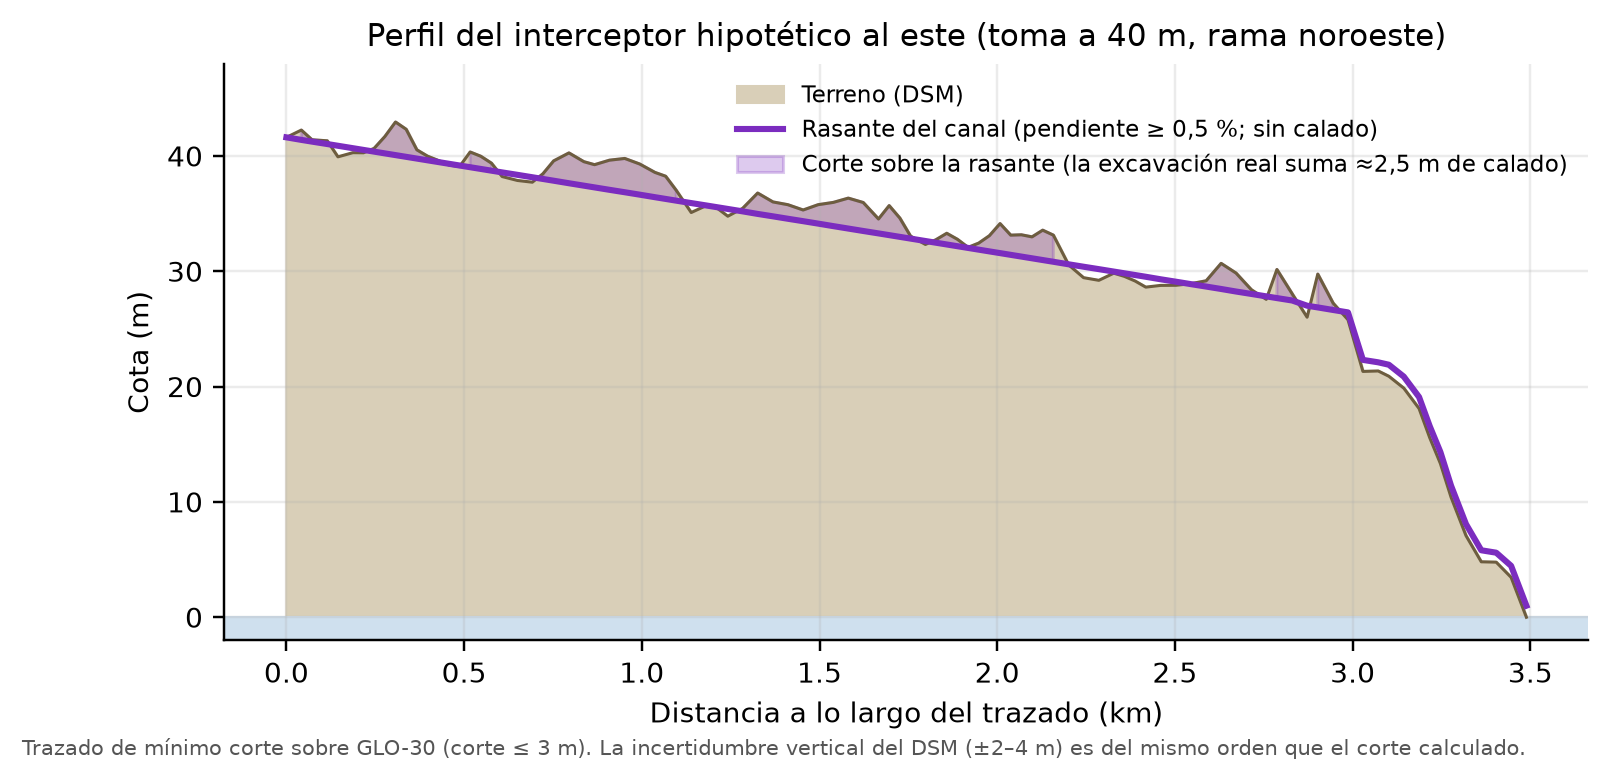
\includegraphics[width=0.9\linewidth]{f_perfil_interceptor.png}
  \caption{Perfil del interceptor hipotético hacia el este (toma en la rama 2 a 40~m): terreno según el DSM, rasante con pendiente $\geq 0,5$\,\% (sin calado) y corte sobre la rasante. En los primeros 2,5~km el desnivel es del orden del error vertical del DSM.}
  \label{fig:interceptor}
\end{figure}

El desvío tampoco actúa sobre la escorrentía local (0,6~km²) ni sobre la falta de salida urbana. No están resueltos el cruce de la rama 1 ni la disipación de energía en el último kilómetro, donde el canal baja unos 29~m hasta el mar. Las vistas tridimensionales de la figura~\ref{fig:3d} muestran la posición del trazado sobre el borde del escarpe, justo encima del vaso.

\begin{figure}[t]
  \centering
  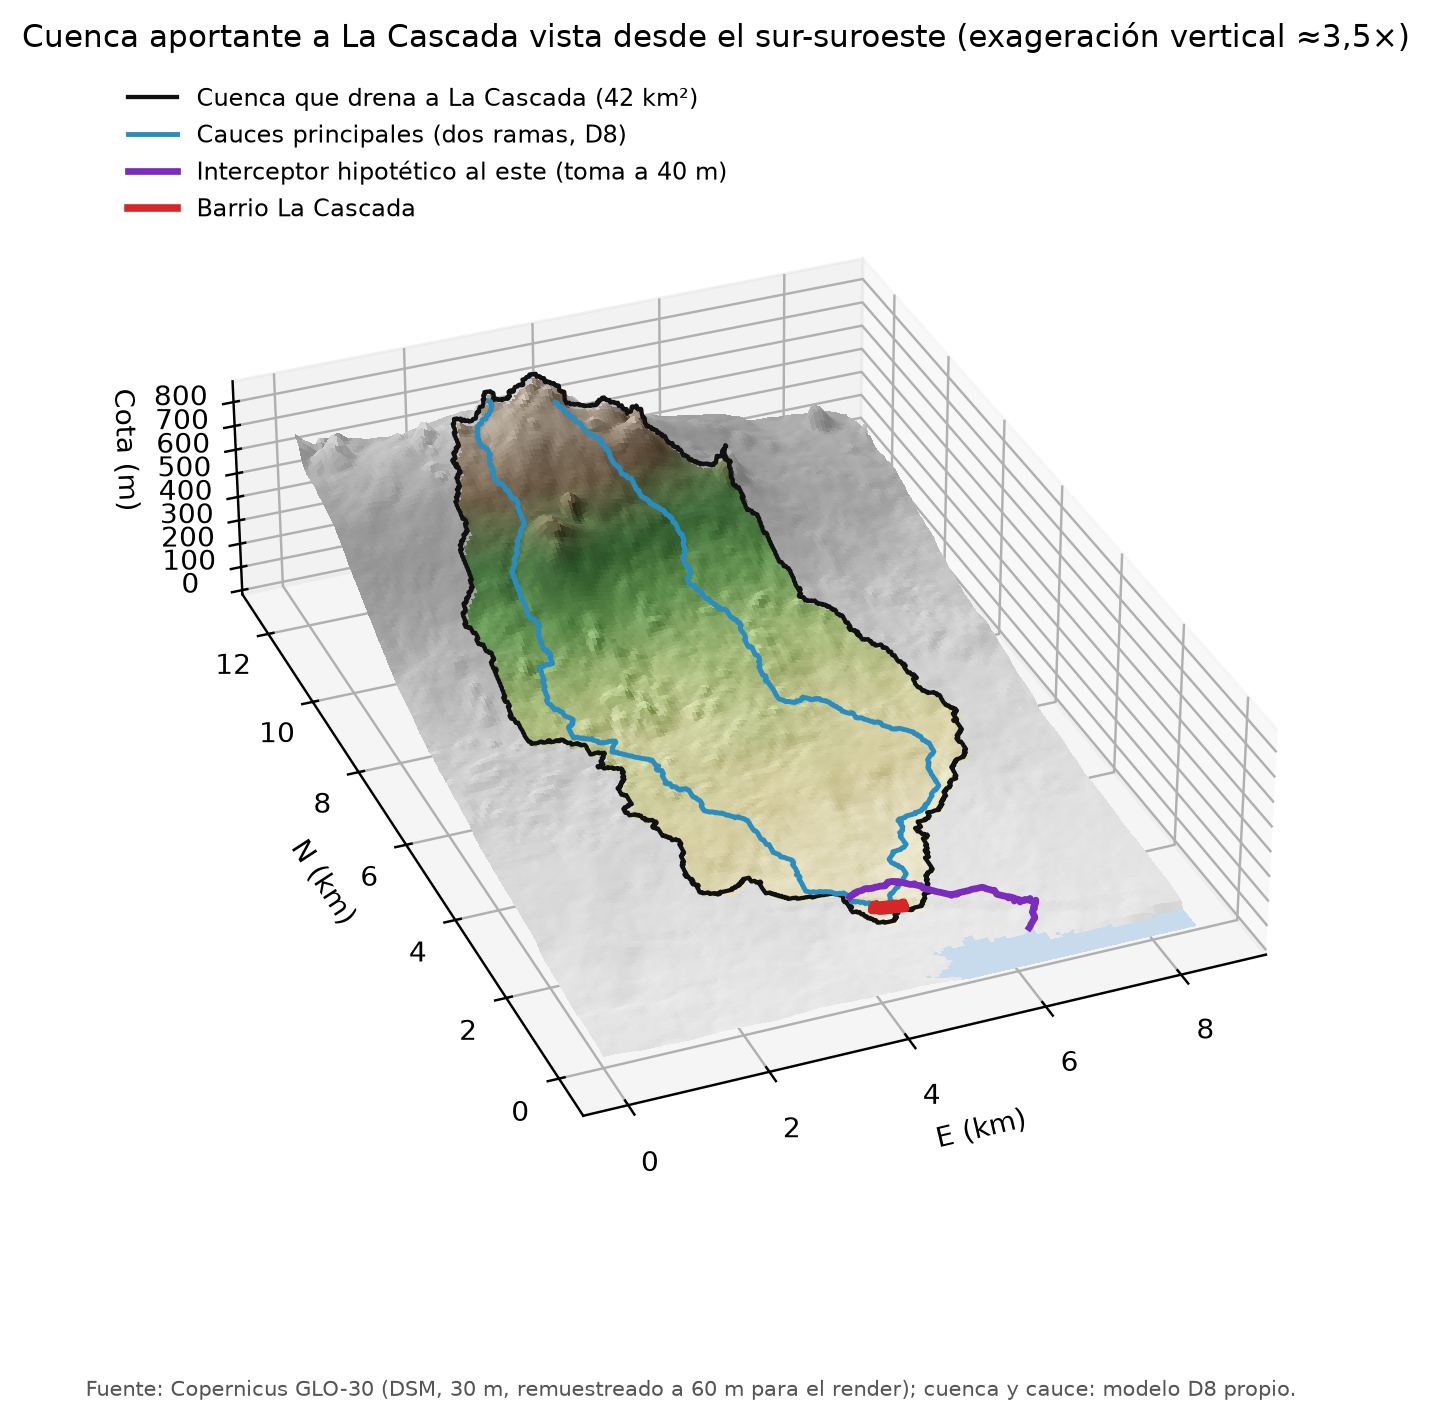
\includegraphics[width=0.49\linewidth]{f3d_cuenca.png}\hfill
  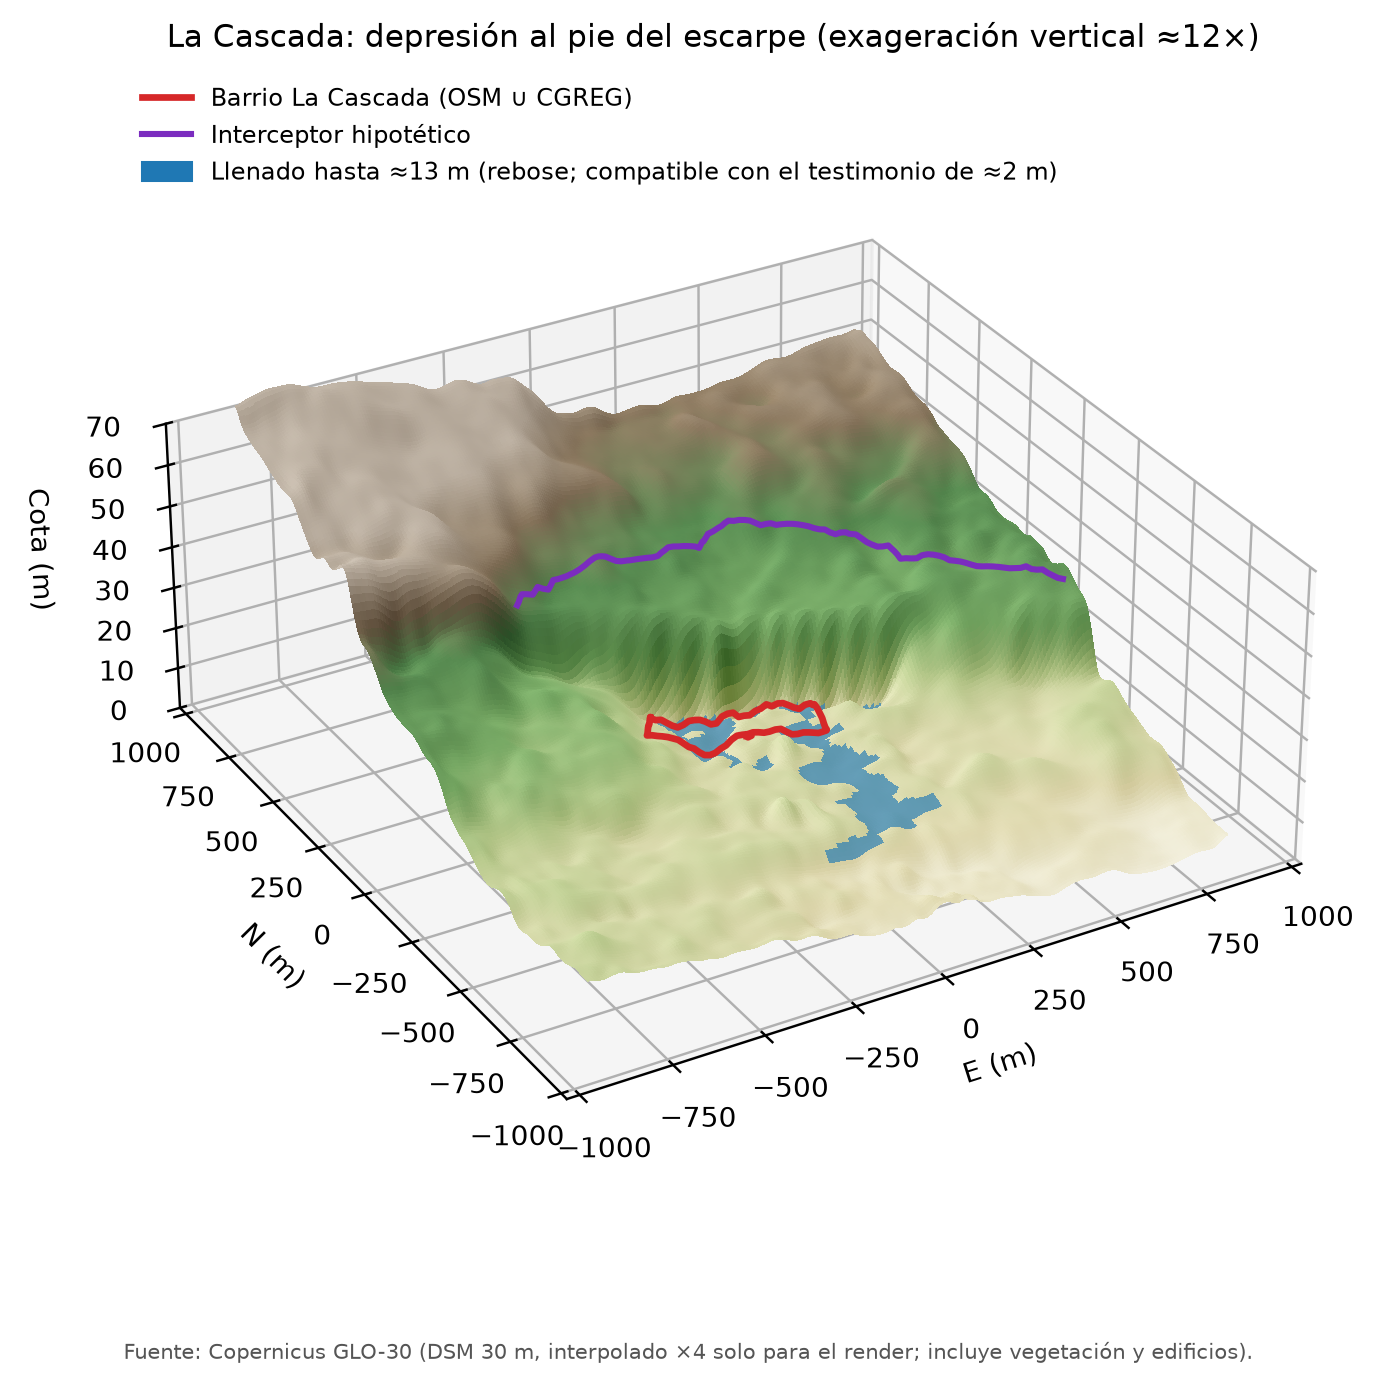
\includegraphics[width=0.49\linewidth]{f3d_barrio.png}
  \caption{Vistas 3D del DSM. Izquierda: cuenca aportante (exageración vertical ${\approx}\,3,5\times$), con el barrio y el interceptor hipotético al este sobre el borde del escarpe (${\approx}\,40$~m). Derecha: entorno de La Cascada (exageración ${\approx}\,12\times$); el barrio ocupa el fondo, al pie del escarpe norte; en morado, el interceptor.}
  \label{fig:3d}
\end{figure}

% =====================================================================
\section{Discusión y limitaciones}

El análisis apunta a un problema de \emph{forma del terreno}: una cuenca de 42~km² descarga en una depresión cerrada de unos 50\,000~m³ sin cauce de salida. Superado el umbral de intensidad, el vaso se llena en horas y lo que fija la altura del agua es cuánta puede salir por la trama urbana. Por eso el SCS-CN, que responde al volumen, y el testimonio de lámina, que responde a la salida, no se pueden usar para calibrarse el uno al otro.

La magnitud del desvío también importa. El pico central medido, de 325--497~m³/s, supera unas 7--14 veces la capacidad de 35--45~m³/s que el estudio urbano atribuye a una calle-canal con colector por la calle Marchena, y supera la capacidad de 150--230~m³/s con la que se evaluó inicialmente el interceptor con la lluvia de ECMWF. Ese rango de caudal es, a la vez, el resultado menos fiable del informe.

\begin{itemize}
  \item \textbf{Terreno.} El error aleatorio del DSM (${\pm}2$~m) es del orden de la profundidad del vaso (2,4~m), de la lámina simulada y del desnivel del interceptor en sus primeros 2,5~km. Los techos y las copas crean umbrales falsos; las grietas y los cauces de menos de 30~m desaparecen. La diferencia entre zona poblada ($-3,4$~m) y no poblada ($-1,9$~m) frente al IGM impide usar cotas absolutas como umbrales.
  \item \textbf{Lluvia.} Dos estaciones útiles, ambas fuera de la cuenca, con totales mínimos por el corte de transmisión a las 21:25. No se sabe si la tormenta cubrió la cumbre. Los pluviómetros de balancín subestiman intensidades de más de 50~mm/h. La serie del INAMHI M0191 en Puerto Ayora no está incorporada (\issue{3}); según el estudio de Santa Cruz, midió unos 135~mm más entre las 22:00 y las 03:00, cuando la red IERSE ya no transmitía.
  \item \textbf{Hidrología.} Modelo agregado, con lluvia uniforme, CN supuestos (el 55 del Parque es un valor de tabla) y sin pérdidas en el cauce. El caudal pico del evento varía en un factor de 2,5 (215--549~m³/s) según la lluvia areal, el CN y el $t_c$, y no hay ningún aforo para contrastarlo.
  \item \textbf{Vaso.} La \enquote{bañera} es estática, y el vertedero de la ecuación~\ref{eq:vertedero} ignora el remanso de los primeros 400~m, casi planos y edificados. $L_w$ es un supuesto. El modelo 2D representa ese remanso \citep{sosg202606}.
  \item \textbf{Desvío.} Los corredores son rasantes, no canales: no incluyen calado, resguardo, disipadores ni estabilidad del terraplén. El encaje legal (DPNG, MAATE, estudio de impacto) no se analizó más allá de la zonificación.
  \item \textbf{Proceso.} El análisis lo hizo un comité de agentes de IA con revisión cruzada; sus discrepancias (volumen del vaso, $t_c$, huso horario de los modelos, lámina y número de familias sin fuente) se resolvieron de forma explícita, pero no hubo verificación de campo.
\end{itemize}

\begin{table}[ht]
  \centering\small
  \caption{Nivel de confianza de cada conclusión.}
  \label{tab:confianza}
  \begin{tabularx}{\linewidth}{>{\raggedright\arraybackslash}Xl}
    \toprule
    Conclusión & Confianza \\
    \midrule
    Área de la cuenca (42,3~km², idéntica con y sin quemar) y sus dos ramas & Alta \\
    Hora del evento (tarde y noche del 30-oct; pico entre las 21:30 y las 23:00) & Alta \\
    Existencia del vaso, rebose a ${\approx}\,12$--13,25~m y salida sin cauce por la ciudad & Media-alta \\
    El vaso se llenó horas antes del pico; la lámina la controla la salida & Media-alta \\
    Lluvia areal del evento (152--208~mm, totales mínimos) & Media-baja \\
    Corredor de desvío al este & Media-baja \\
    Caudales pico & Baja (orden de magnitud) \\
    \bottomrule
  \end{tabularx}
\end{table}

% =====================================================================
\section{Conclusiones y trabajo futuro}
\begin{enumerate}
  \item Al barrio La Cascada drenan 42,3~km², casi toda la cuenca de Puerto Ayora, por dos quebradas que terminan en su borde norte.
  \item El barrio es un vaso cerrado al pie de escarpes, con fondo a 10,5~m, rebose a 12,0--13,25~m (DSM) y 42\,000--62\,000~m³ de almacenamiento. Entre él y el mar no hay cauce: la salida natural cruza la ciudad con ${\approx}\,1$\,\% de pendiente.
  \item Con la lluvia medida del 30-oct, la escorrentía fue de 46 a 92 veces el vaso, que se habría llenado entre las 15:40 y las 20:00 (todos los escenarios); el pico, de 215 a 549~m³/s, llegó entre las 21:30 y las 22:50. La altura del agua la controla la salida.
  \item El desvío al este no es descartable, pero no está demostrado: su pendiente inicial está dentro del error del DSM, exigiría terraplén alto o corte profundo en basalto sobre el escarpe y quedaría entero en el Parque Nacional. Hacia el oeste no es viable.
  \item Los resultados no justifican tratar el desvío como medida de emergencia. El propio comité de agentes propuso tratarlo como una alternativa más, junto con la salida urbana, la laminación, la regulación del suelo y la reubicación voluntaria.
\end{enumerate}

Para pasar del reconocimiento a una decisión hacen falta:
\begin{itemize}
  \item marcas de agua y cota real del rebose con GNSS (\issue{2}, \issue{65});
  \item un modelo del terreno de dron o LiDAR de 5--10~km² del escarpe, el barrio y el corredor este (\issue{16});
  \item la lluvia del INAMHI M0191 incorporada al estudio (\issue{3}) y pluviómetros en la cuenca (\issue{19});
  \item aforos o huellas de crecida en las quebradas (\issue{9}) y ensayos de infiltración (\issue{10});
  \item el catastro de sumideros y pasos bajo vías (\issue{5}), y el historial de OSM y las fotografías aéreas del IGM para el supuesto cauce este (\issue{11});
  \item confirmar si hubo inundación el 3-oct (\issue{52}), y un modelo lluvia--caudal y 2D calibrados (\issue{25}, \issue{26}).
\end{itemize}

\section*{Disponibilidad de datos y código}
{\small\sloppy Todo el cálculo es reproducible desde el repositorio público \emph{mayait/sosgalapagos-datos}, en la carpeta \texttt{geodatos/}:
\begin{itemize}
  \item \texttt{scripts/12\_cascada\_analisis.py}: cuenca, vaso, curva cota--volumen, rebose, corredores, hidrogramas y \texttt{resumen.json};
  \item \texttt{scripts/13\_cascada\_figuras.py}: las figuras del estudio;
  \item \texttt{scripts/14\_cascada\_informe.py}: el PDF preliminar de 39 páginas a partir de \texttt{estudios/la-cascada/texto/}.
\end{itemize}
Los resultados están en \texttt{geodatos/estudios/la-cascada/datos/}: \texttt{resumen.json}, \texttt{curva\_cota\_volumen.csv}, \texttt{hidrogramas\_evento\_30oct.csv}, \texttt{rutas\_desvio.geojson} y \texttt{perfil\_interceptor\_este.csv}, entre otros. La figura~\ref{fig:transito} se genera con \texttt{informes/2026-04-la-cascada/figuras.py}. Los datos crudos (\texttt{geodatos/descargas/}) no se publican porque algunas capas oficiales contienen datos personales; se regeneran con los scripts \texttt{01}--\texttt{07}. Este informe se compila con \texttt{informes/compilar.sh 2026-04-la-cascada}.\par}

\bibliographystyle{sosg}
\bibliography{referencias,bib-2026-04}

\end{document}
